Pierwszym krokiem algorytmu wykrywania logo \bk, jest przetwarzanie wstępne. Celem przetwarzania wstępnego jest zmniejszenie rzeczywistego rozmiaru, poprawa jakości obrazu oraz usunięcie zakłóceń.

\subsection{Skalowanie obrazu}
Celem skalowania obrazu jest stworzenie nowego obrazu o~zmienionym rozmiarze, wykorzystując do tego obraz oryginalny. W~przypadku projektowanego systemu, obraz analizowany jest poddawany skalowaniu aby zmniejszyć jego rzeczywisty rozmiar, celem uproszczenia dalszych obliczeń.

Do zmiany rozdzielczości obrazu cyfrowego zwykle wykorzystuje się metody interpolacji. Algorytmy tego typu można podzielić na algorytmy nieadaptacyjne oraz adaptacyjne. Pierwsza grupa dokonuje interpolacji w~ustalony z~góry sposób, niezależnie od zawartości przetwarzanego obrazu. Algorytmy adaptacyjne zmieniają sposób przetwarzania pikseli, biorąc pod uwagę cechy aktualnie przetwarzanego fragmentu. Adaptacja pozwala na zwiększenie jakości wizualnej, zwiększając przy tym koszt obliczeniowy~\cite{swierczynski2008podwyzszanie}.

\subsubsection{Interpolacja dwuliniowa}
Algorytm interpolacji dwuliniowej jest algorytmem nieadaptacyjnym, nieco bardziej zaawansowanym niż pokrewny algorytm najbliższego sąsiada. Wartość każdego piksela obrazu wynikowego jest obliczana na podstawie czterech sąsiednich punktów obrazu wejściowego~\cite{algorytmy:bilinear}.

W~pierwszym kroku algorytmu oblicza się w~którym miejscu w~obrazie wejściowym znajduje się rozpatrywany punkt obrazu wyjściowego. Dokonuje się tego poprzez obliczenie współczynników skalowania, zgodnie z~wzorami~\ref{eqn:wsp-skalowania-x}~i~\ref{eqn:wsp-skalowania-y}.

\begin{equation}
    \label{eqn:wsp-skalowania-x}
    r_{x} = \frac{\mathrm{width}_{input}}{\mathrm{width}_{output}}
\end{equation}

\begin{equation}
    \label{eqn:wsp-skalowania-y}
    r_{y} = \frac{\mathrm{height}_{input}}{\mathrm{height}_{output}}
\end{equation}

Na podstawie współczynników $r_{x}, r_{y}$ dla piksela $(i, j)$ obrazu wyjściowego oblicza się pozycję~$(x, y)$ w~obrazie wejściowym, wykorzystując zależność \ref{eqn:skalowanie}.

\begin{equation}
    \label{eqn:skalowanie}
    \begin{array}{ll}
        x = i \cdot r_{x} & y = j \cdot r_{y}
    \end{array} 
\end{equation}

Na podstawie informacji o~docelowym punkcie, wybiera się cztery najbliższe punkty $F_{0,0}, F_{0,1}, F_{1,0}, F_{1,1}$, podobnie jak na~\ref{fig:bilinear-result} (żółtym kolorem zaznaczono punkt obliczony z~wzorów~\ref{eqn:skalowanie}). 

\begin{figure}[h]
    \centering
    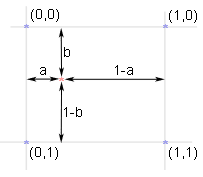
\includegraphics[width=0.6\columnwidth]{figures/bi2.png}
    \caption{Dobór sąsiednich punktów w~algorytmie interpolacji dwuliniowej~\cite{algorytmy:bilinear}}
    \label{fig:bilinear-result}
\end{figure}

Następnie trzykrotnie przeprowadza się interpolację pomiędzy punktami, najpierw dwa razy w~kierunku poziomym pomiędzy $F_{0,0}$~i~$F_{1,0}$ oraz $F_{0,1}$~i~$F_{1,1}$ i~ostatni raz pomiędzy wynikami poprzednich interpolacji, zgodnie ze wzorem~\ref{eqn:interpolacja}.
Proces ten należy powtórzyć dla każdej składowej koloru z~osobna~\cite{algorytmy:bilinear}.

\begin{equation}
    \label{eqn:interpolacja}
    \begin{array}{l}
        F_{a,0} = (1-a) \cdot F_{0,0} + a \cdot F_{1,0} \\
        F_{a,1} = (1-a) \cdot F_{0,1} + a \cdot F_{1,1} \\
        F_{a,b} = (1-b) \cdot F_{a,0} + b \cdot F_{0,1} \\
    \end{array} 
\end{equation}

W~stworzonym rozwiązaniu, algorytm interpolacji dwuliniowej jest implementowany przez  obiekty klasy \texttt{POBR::BilinearInterpolationResizer}. Wyniki działania tego algorytmu zostały przedstawione na rysunku~\ref{fig:bilinear-result}. 
\begin{figure}%
    \centering
    \subfloat[800x800px]{{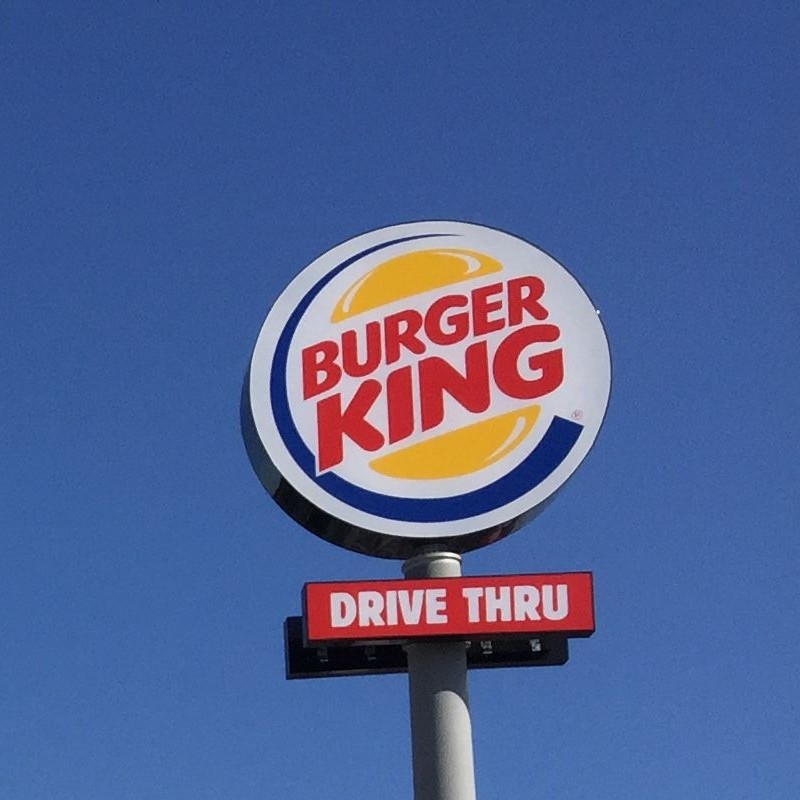
\includegraphics[scale=0.16]{./figures/ikonka.jpg} }}%
    \qquad
    \qquad
    \subfloat[400x400px]{{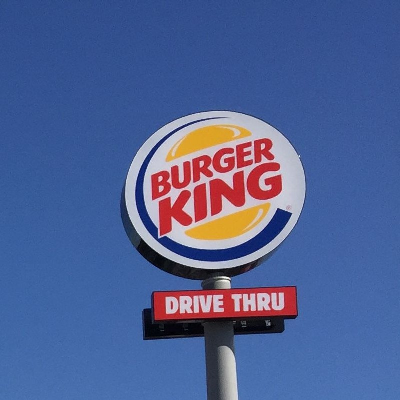
\includegraphics[scale=0.16]{./figures/ikonka_rev.png} }}%
    \caption{Efekt działania algorytmu interpolacji dwuliniowej na przykładzie zmniejszania logo \bk z~rozmiaru 800x800px do 400x400px}%
    \label{fig:bilinear-result}%
\end{figure}

\subsubsection{Interpolacja z uwzględnianiem krawędzi}
\todo{Opisać adaptacyjny algorytm interpolacji z uwzględnieniem krawędzi.}

\subsection{Filtracja zakłóceń}
\todo{Opisać algorytm filtracji zakłóceń - filtracja medianowa. Znaleźć źródła.}